\documentclass [xcolor=svgnames, t, 9pt] {beamer} 

\usepackage[utf8]{inputenc}
\usepackage{booktabs, comment} 
\usepackage[absolute, overlay]{textpos} 
\usepackage{pgfpages}
\usepackage[font=footnotesize]{caption}
\useoutertheme{infolines} 
\usepackage[final]{graphicx}

\definecolor{gold}{RGB}{219, 170, 50}

\setbeamercolor{title in head/foot}{bg=gold, fg=black}
\setbeamercolor{author in head/foot}{bg=myuniversity}
\setbeamertemplate{page number in head/foot}{}
\usepackage{csquotes}
 \usepackage{color}

\usepackage{amsmath}
\usepackage[makeroom]{cancel}


\usepackage{textpos}

\usepackage{tikz}

\usetheme{Madrid}
\definecolor{myuniversity}{RGB}{22, 77, 166}
\usecolortheme[named=myuniversity]{structure}
\usepackage{tikz}



\title[MDI using SAE methods]{Multidimensional deprivation index using small area estimation methods: }
\subtitle{An application for the adult population in Colombia}
\institute[]{}
\titlegraphic{
\includegraphics[height=1.5cm]{Bild 23.09.22 um 10.31.jpg}}
\author[Alejandra Arias-Salazar]{
	Andrés Gutiérrez\textsuperscript{1},
	Alejandra Arias-Salazar\textsuperscript{2},
Stalyn Guerrero-Gómez \textsuperscript{1},
	Natalia Rojas-Perilla\textsuperscript{3} ,
	Xavier Mancero\textsuperscript{1},
Hanwen Zhang\textsuperscript{4}}


\institute[]{Economic Commission for Latin America and the Caribbean^{1}\\
Freie Universität Berlin^{2}\\
United Arab Emirates University^{3}\\
 Universidad Autónoma de Chile^{4}}
\date{}


\addtobeamertemplate{navigation symbols}{}{%
    \usebeamerfont{footline}%
    \usebeamercolor[fg]{footline}%
    \hspace{1em}%
    \insertframenumber/\inserttotalframenumber
}

\begin{document}
\begin{frame}
\maketitle
\end{frame}


%%%%%%%%%%%%%%%%%%%%%%%%%%%%
%\logo{\includegraphics[height=1cm]{logo.jpg}~%
%}


%%%%%%%%%%%%%%%%%%%%%%%%%%



\begin{frame}
\frametitle{Table of Contents}
\tableofcontents
\end{frame}

\section{Motivation}
\begin{frame}{Motivation}

   \vspace{0.5cm}
\begin{itemize}
    \item Poverty and multidimensional poverty leading topics in national and international agendas: ``End poverty in all its forms everywhere" (UN General Assembly, 2015).
\end{itemize}

\begin{figure}[!htb]
\centering
\subfigure
\includegraphics[width=0.3\linewidth]{logo_sdgs.jpg}
\subfigure
\includegraphics[width=0.15\linewidth]{goal1.png}
\end{figure}

\begin{itemize}
    \item Necessity of quality data on poverty in its different expressions. 
    
    \vspace{0.5cm}
    
    \item Disaggregated information: geographically and based on relevant characteristics (e.g. sex, age, ethnicity) 
\end{itemize}

\end{frame}


\section{Case study: Multidimensional deprivation index in Colombia}




\begin{frame}{The ECLAC multidimensional deprivation index (MDI)}

\begin{itemize}
    \item ECLAC is developing a regionally comparable MDI for 18 Latin American countries.
\item The index considers the person (and not the household) as unit of analysis. 
%\item This case study is based on the application of such index to the adult population in Colombia.
\item The MDI is based on the Alkire \& Foster (2007) methodology.
\item Complements the Global Multidimensional Poverty Index using regionally specific indicators and thresholds. 

\pause 
\item  It considers 5 dimensions and 8 indicators:

\vspace{0.1cm}

\begin{table}[ht]
	\begin{center}
	\scriptsize{
			\centering
			\begin{tabular}{llccc}
		
				\hline
					&&&&&
				\textbf{Dimension} & \textbf{Indicator}& \textbf{Weight} &\textbf{Available in census} &\textbf{Target population} 
	&&&&&
					\\
				\hline
				&&&&&
				Housing &Poor housing materials & 1/10 & Yes & Adults and seniors\\

				& Overcrowding & 1/10 &Yes & Adults and seniors \\
	&&&&&
						
				\hline
					&&&&&
				Water and sanitation 
				& Lack of drinking water & 1/10 &Yes & Adults and seniors 
				\\
				& Lack of sanitation &1/10 & Yes & Adults and seniors \\
	&&&&&
					\hline
	&&&&&				Energy and connectivity  
				& 
				 Lack of internet service & 1/10 &Yes & Adults and seniors \\
				
				& Lack of electricity & 1/10 &Yes & Adults and seniors \\
				&&&&&
				\hline
					&&&&&
				Education & Unfinished education & 2/10 &\textbf{No*} &Adults and Seniors\\
	&&&&&
				\hline
					&&&&&
				Employment and social  & No or insufficient pension & 2/10 & \textbf{No} & Seniors \\
			  protection & Unemployment or insufficient &2/10 & \textbf{No} &Adults\\
			   &employment-related income  &&&\\
			   	&&&&&
				\hline
			\end{tabular}
		}
	\end{center}
\end{table}

\end{itemize} 

\end{frame}

\begin{frame}{The ECLAC multidimensional deprivation index (MDI)}
    \vspace{0.3cm}
    
The MDI is computed as: 

\begin{equation}
    \text{MDI}_d =\frac{1}{N_d} \sum^{N_d}_{j=1} I(q_{dj} > z)
\end{equation}

The indicator function $I(\cdot)$ equals 1 when the condition $q_{dj} > z$ is met, i.e. $q_{dj} > 0.4$. 

\vspace{0.3cm}

$q_{dj}$ is a weighted quantity considering the $k=8$ indicators that comprise the index. 

\vspace{0.3cm}
$$ q_{dj} = 0.1  \sum^{6}_{k=1} y_{dj}^k + 0.2 \sum^{8}_{k=7} y_{dj}^k$$

\vspace{0.3cm}

$y_{dj}^k$ indicates if the person $j$ in domain $d$ has a deprivation or not in each of the $k=8$ indicators. 

\end{frame}



\begin{frame}{Case study: Multidimensional deprivation index in Colombia}


\begin{figure}[htp]
    \centering
    \includegraphics[width=10cm]{6a.png}\hspace*{-1cm}
    \caption{Direct estimates of MDI components for 6 available indicators at municipality level.}
\end{figure}


\end{frame}

\begin{frame}{Case study: Multidimensional deprivation index in Colombia}

\vspace{0.3cm}

\begin{itemize}
\item \textbf{Objective:} Producing reliable estimates of the multidimensional deprivation index and its components (indicators and dimensions) for the adult population of Colombia at first (departments) and second administrative division (municipalities). 

%\vspace{0.2cm}
%\pause
%\begin{itemize}
%    \item 27\% departments and 61\% municipalities out-of-sample.
%    \vspace{0.2cm}
%    \pause 
%    \item For the in-sample municipalities, around 6\% of the domains have coefficient of variation higher than 15\% in both indicators.
%\end{itemize}

\pause
\vspace{0.3cm}

\item \textbf{Challenge:} 2/8 indicators are missing so the final MDI cannot be computed.

\pause

\vspace{0.3cm}

\item \textbf{Identified scenarios:} 
\begin{itemize}
\vspace{0.3cm}
    \item \textbf{Only 1 missing indicator:} Using a unit-level Bernoulli logit mixed model.% for both missing indicators.
    \pause
\vspace{0.3cm}
    \item \textbf{Two missing indicators:} Finding the the expected value of the linear combination of the them.
    \pause
\vspace{0.3cm}
    \item \textbf{More than two missing indicators:} Using a Monte Carlo simulation approach to obtain ``hard" estimates (0,1) for each individual in each missing indicator.
\end{itemize}  %The goal is not obtaining summary statistics for each indicator 

\vspace{0.3cm}

\pause

\item \textbf{Assumptions:} There is no dependence when there are two or more missing indicators, and there are no causal relationships between the dependent and independent variables.
\end{itemize}
\end{frame}


\section{Methodology}


\frame[noframenumbering]{\tableofcontents[currentsection,hideothersubsections,currentsubsection]}

\begin{frame}{Unit-level Bernoulli logit mixed model}

\begin{itemize}
    \item The variable of interest is binary ($y_{dj} =0$ or $1$), 
 \vspace{0.5cm}   
    \item The target estimation can be, the proportion per domain: 
$\bar{Y}_d = \pi_d = \frac{1}{N_d} \sum_{j=1}^{N_d} y_{dj}$, with $j=1, \dots, N_d$, $d=1, \dots, D$, and $\pi_{dj}$ the probability that a specific unit $j$ in the domain $d$ obtains the value 1. 

\pause

\vspace{0.5cm}

\item The generalized linear mixed model (GLMM) with a logit link function is defined as: 

    \begin{equation*}\label{eq:Plugin1}
        \text{logit}(\pi_{dj}) = \text{log} \Big (   \frac{\pi_{dj}} {1-\pi_{dj}} \Big) = \eta_{dj} = x^T_{dj}\beta + u_d,
    \end{equation*}

with  $\beta$ the vector of fixed-effects parameters, $u_d$ the random area-specific effect for $d$ and $u_d \sim N(0,\sigma_u^2)$.
\vspace{0.5cm}
\item $u_d$ are assumed independent with $y_{dj}|u_d \sim \text{Bernoulli}(\pi_{dj})$ with $E(y_{dj}|u_d) = \pi_{dj}$ and $Var(y_{dj}|u_d) = \sigma_{dj}=\pi_{dj}(1-\pi_{dj})$.
\end{itemize}
\end{frame}



\begin{frame}{Point estimation - one missing indicator}

\vspace{0.3cm}

The plug-in predictor of $\pi_{dj}$ is:
       
       \begin{equation}
           \hat{\pi}^{in}_{dj} = \frac{\text{exp}(\bold{x}^{T}_{dj}\hat{\beta}+\hat{u}_d)} {{1+\text{exp}(\bold{x}^{T}_{dj}\hat{\beta}+\hat{u}_d)}},
       \end{equation}

\vspace{0.5cm}
       
which would allow obtaining the plug-in predictor of $\bar{Y}_d$:

\vspace{0.3cm}

\begin{equation}
    \hat{\bar{Y}}^{in}_{d} = \frac{1}{N_d} \big( \sum_{j \in s_d} y_{dj} + \sum_{j \in r_d} \hat{\pi}^{in}_{dj} \big), 
\end{equation}

\vspace{0.3cm}

where $s$ and $r$ represent the in- and out-of-sample observations respectively.
\pause

\vspace{0.5cm}

* In this case study, the two missing indicators $Y_{1}$ = \textit{education} and $Y_{2}$= \textit{employment} could be obtained with this procedure. \textbf{However, it does not allows to compute the final MDI.}

%\pause

%\vspace{0.5cm}

%* Find the probability mass function of the linear combination of both random variables with the existing indicators:
%$$X_{j}=\alpha\left(Y_{1j}+Y_{2j}\right)+k_{j}$$.



\end{frame}


\begin{frame}{Point estimation - two missing indicators}\label{point}

\vspace{0.2cm}
    
Let's define the poverty status for each individual $j$, i.e. multidimensional poor (1) or not (0) based on a threshold $\delta$: 

\[
Z_{j}=\begin{cases}
1 & \text{if }X_{j}\geq\delta,\\
0 & \text{if }X_{j}<\delta
\end{cases}
\]

\vspace{0.1cm}
\pause 
where 
\[X_{j}=\underbrace{\alpha\left(Y_{1j}+Y_{2j}\right)}_{\mathclap{\text{$W_j$ unknown}}} + \underbrace{k_j.}_{ \mathclap{\text{known}}} \]

\vspace{0.2cm}
\pause 

By finding the mass probability function of $W_j$, the domain proportion is:

\vspace{0.2cm}

$$\bar{Z}_{d}=\frac{1}{N_{d}}\sum_{j\in U_{d}}Z_{j}.$$

\vspace{0.2cm}

The target predictor is then the estimator of $\bar{Z}_{d}$, which is given by the expectation of $\bar{Z}_{d}$:
$$\widehat{\text{MDI}}_d = \hat{\bar{Z}}_{d} = E\left(\bar{Z}_{d}\right)$$

    \hyperlink{AppendixA}{\beamergotobutton{Details}}
\end{frame}






\begin{frame}{Point estimation - more than two missing indicators} %- Monte Carlo approach}

A Monte Carlo simulation approach can be implemented when more than three indicators are missing: 
    \vspace{0.5cm}
    
%The steps to obtain ``hard" estimates (0,1) of the \textbf{education $k=1$ and employment indicator $k=2$ for each individual $j$} in the census are: 

\begin{enumerate}
    \item  Use the sample data to fit a unit-level Bernoulli logit mixed model for each indicator and estimate $\hat{\beta}^k$, $\hat{u}^k_d$, and finally $\hat{\pi}^{in,k}_{dj}$. 
    
    \vspace{0.3cm}

\item for $l = 1, \dots, L$ Monte Carlo simulations:
    \vspace{0.3cm}
\begin{itemize}

    \item For each individual in the census, predict the probability of obtaining the value 1. i.e. $\hat{\pi}^{in,k, (l)}_{dj} \hspace{5} \forall \hspace{5} j \in U_d$.
    \vspace{0.2cm}
    
    \item Obtain Monte Carlo ``hard" estimates $\tilde{y}^{k, (l)}_{dj}$ with $y^k_{dj}  \sim \text{Bernoulli}(\hat{\pi}^{in,k}_{dj})$.
    \vspace{0.2cm}
    
\item Compute the $\text{MDI}^{(l)}$, with 6/8 indicators already available in the census and the new indicators $\tilde{y}^{k,(l)}_{dj}$. %where $k=1$ is the \textbf{education} indicator and $k=2$ the \textbf{employment} indicator.

    
\end{itemize}
    \vspace{0.3cm}
\item The final point estimate in each small area $d$ is computed by taking the mean over each $L$ simulation: $$\widehat{\text{MDI}}_d = \frac{1}{L} \sum^L_{l=1}\text{MDI}^{(l)}_d$$

\end{enumerate}
%\begin{overlayarea}{\textwidth}{\textheight}
%\lipsum[3]\renewcommand{\ReturnTo}{point}

%\hfill\hyperlink{sec:AppendixA}{\beamergotobutton{details}}
%\end{overlayarea}


\end{frame}





\begin{frame}{Uncertainty estimation: Following González-Manteiga et al (2007)}

\begin{itemize}
    \item Suitable when using a logistic mixed model for estimating any characteristic
of the population.
\vspace{0.1cm}
\item Small area robust wild bootstrap (SAWB) is a re-sampling procedure for the MSE estimation of an empirical predictor. 

\vspace{0.2cm}
\end{itemize}

\pause

	\begin{enumerate}
		\item
		For $k = 1,2$
		\item
		For $b = 1,...,B$
		\begin{itemize} 
			\item Using the already estimated $\hat{\beta}^k, \hat{\sigma}^{2,k}_u$, generate $u_{d}^{*,k}$ and simulate a bootstrap superpopulation $y^{k,(b)}_{dj}  \sim \text{Bernoulli}({\pi}^{*,k}_{dj})$ with $   {\pi}^{*,k}_{dj} = \frac{\text{exp}(\bold{x}^{T}_{dj}\hat{\beta}+{u}_{d}^{*})} {{1+\text{exp}(\bold{x}^{T}_{dj}\hat{\beta}+{u}_{d}^{*})}}$

			\item Calculate the $\text{MDI}_{d}^{(b)}$ 
			
			\vspace{0.3cm}
			
			\item Extract the bootstrap sample and obtain the estimated MDI following the point estimate - Monte Carlo approach  $\widehat{\text{MDI}}_{d}^{(b)}$
		\end{itemize}
		\vspace{0.2cm}

		\item	
		$
		\text{MSE}\Big[ \widehat{\text{MDI}}_{d} \Big]=1/B \sum\limits_{b=1}^{B}\Big[\text{MDI}_{d}^{(b)}-\widehat{\text{MDI}}_{d}^{(b)}\Big]^2
		$		
	\end{enumerate}

\end{frame}


\section{Application}


\frame[noframenumbering]{\tableofcontents[currentsection,hideothersubsections,currentsubsection]}


\subsection{Data sources}

\begin{frame}{Data sources and covariates}

\vspace{0.5cm}

\textbf{Data sources:}

\begin{itemize}
    \item National population and housing census, Colombia 2018.
    \item Employment and living conditions survey (Large Integrated Household Survey), Colombia 2018.
    \item Satellite imagery, Colombia 2016 from Earth Engine Data Catalog.
\end{itemize}


\vspace{0.5cm}

\pause 

\textbf{Covariates:}

\vspace{0.3cm}

\begin{minipage}[t]{0.45\textwidth}
Census and survey data
\begin{itemize}
\item Group of age
\item Area (urban/rural)
\item Department 
\item Sex
\item 6 $y^k_{dj}$ ($k=$ water, energy, housing material, sanitation, overcrowding, internet)
\end{itemize}
\end{minipage}
\begin{minipage}[t]{0.45\textwidth}
Satellite imagery 
\begin{itemize}
\item Intensity of nighttime lights 
\item Distance to cultivated areas (crops) 
\item Urbanization (human settlements)
\end{itemize}

\vspace{0.2cm}
Area level

\begin{itemize}
\item Unemployment rate 
\end{itemize}
\end{minipage}
\end{frame}

\subsection{Results}


\begin{frame}{Results: Estimated MDI indicators}


\begin{figure}[htp]
    \centering
    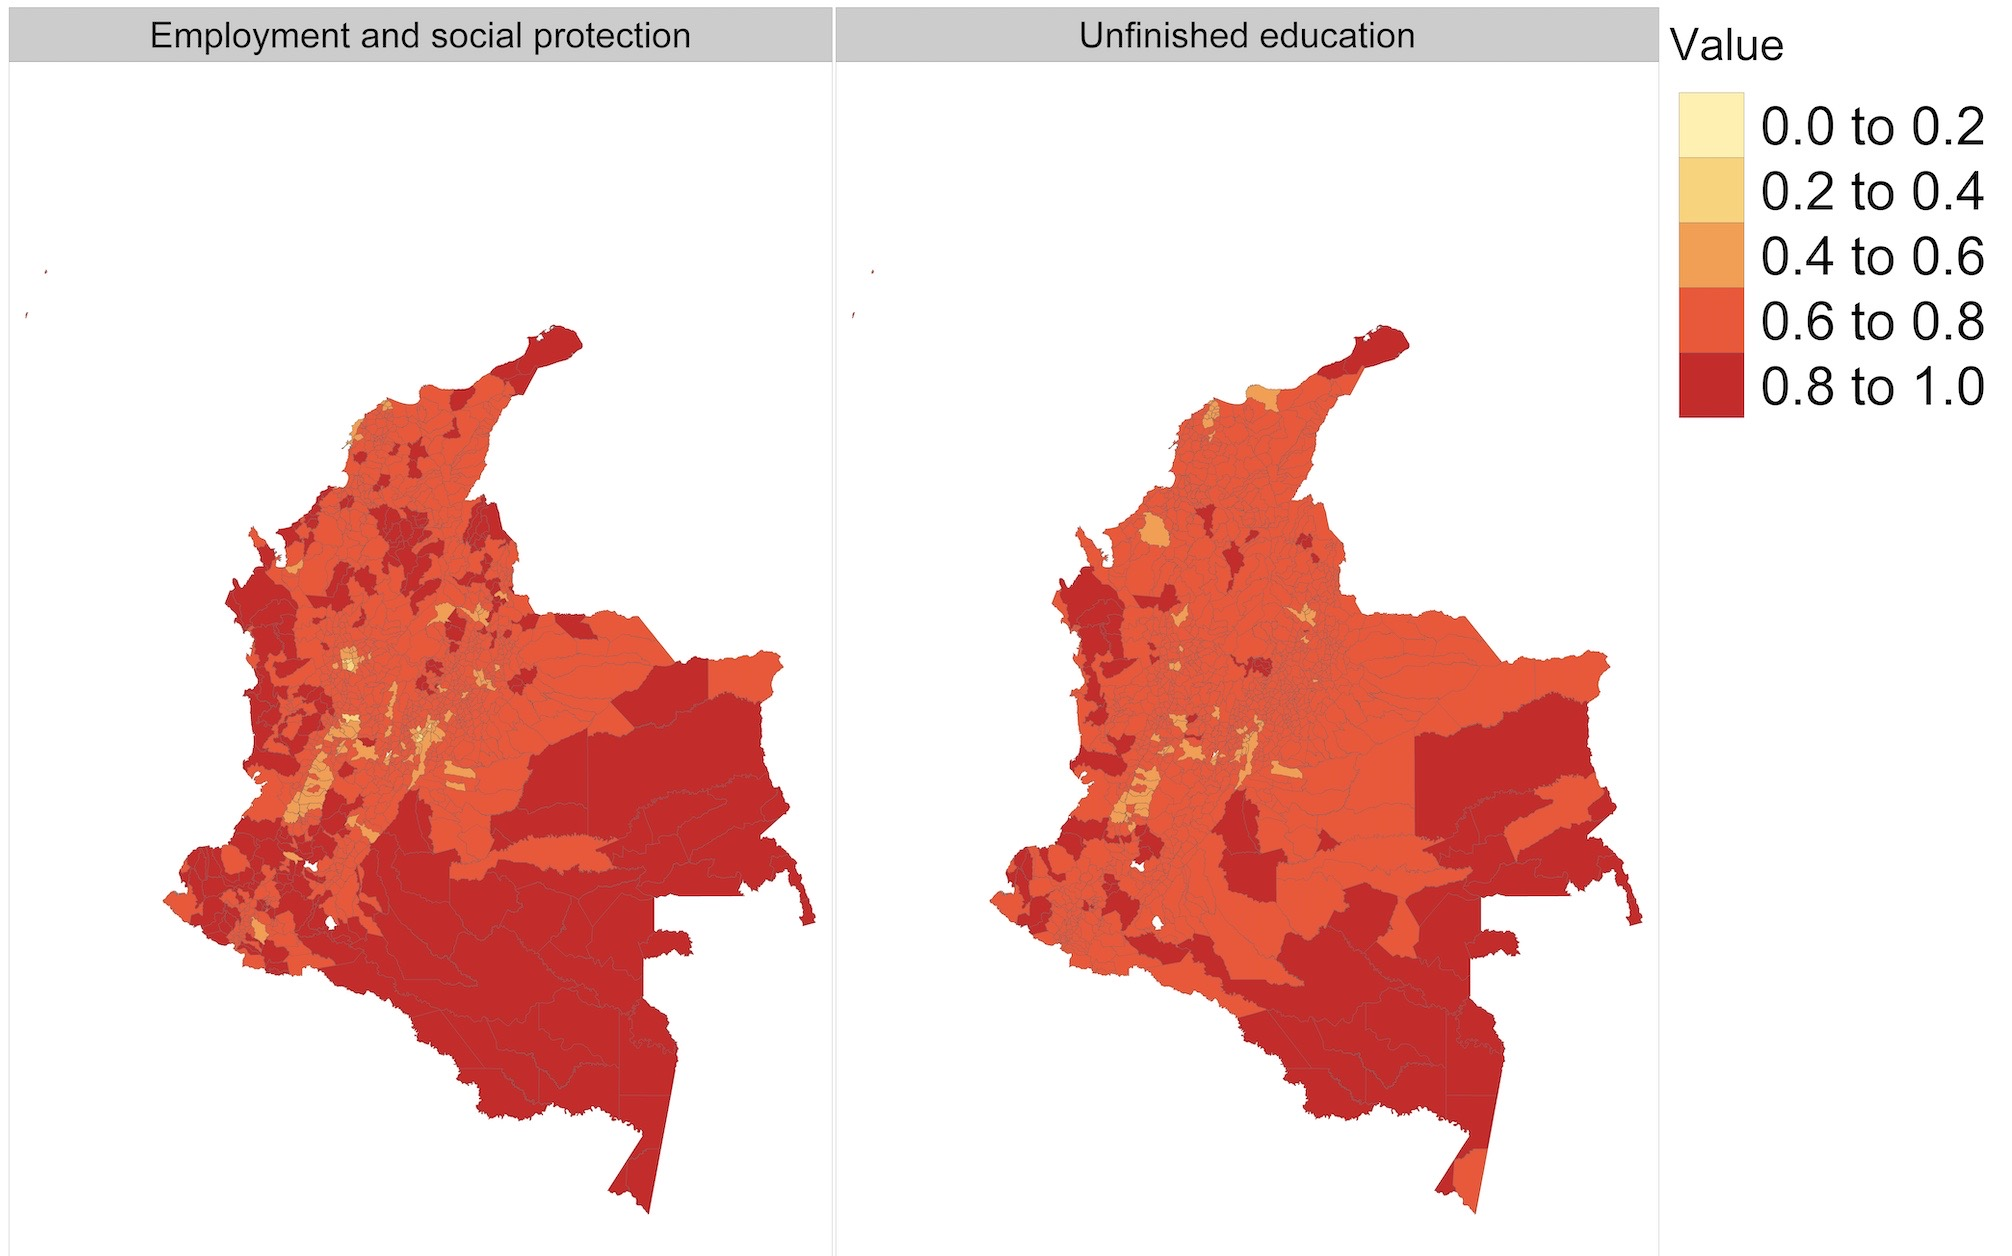
\includegraphics[width=10cm]{6b.jpg}\hspace*{-1cm}
    \caption{Model-based estimates for the indicators employment and social protection and unfinished education at municipality level.}
\end{figure}


\end{frame}







\begin{frame}{Results: Estimated MDI}


\begin{figure}[htp]
    \centering
    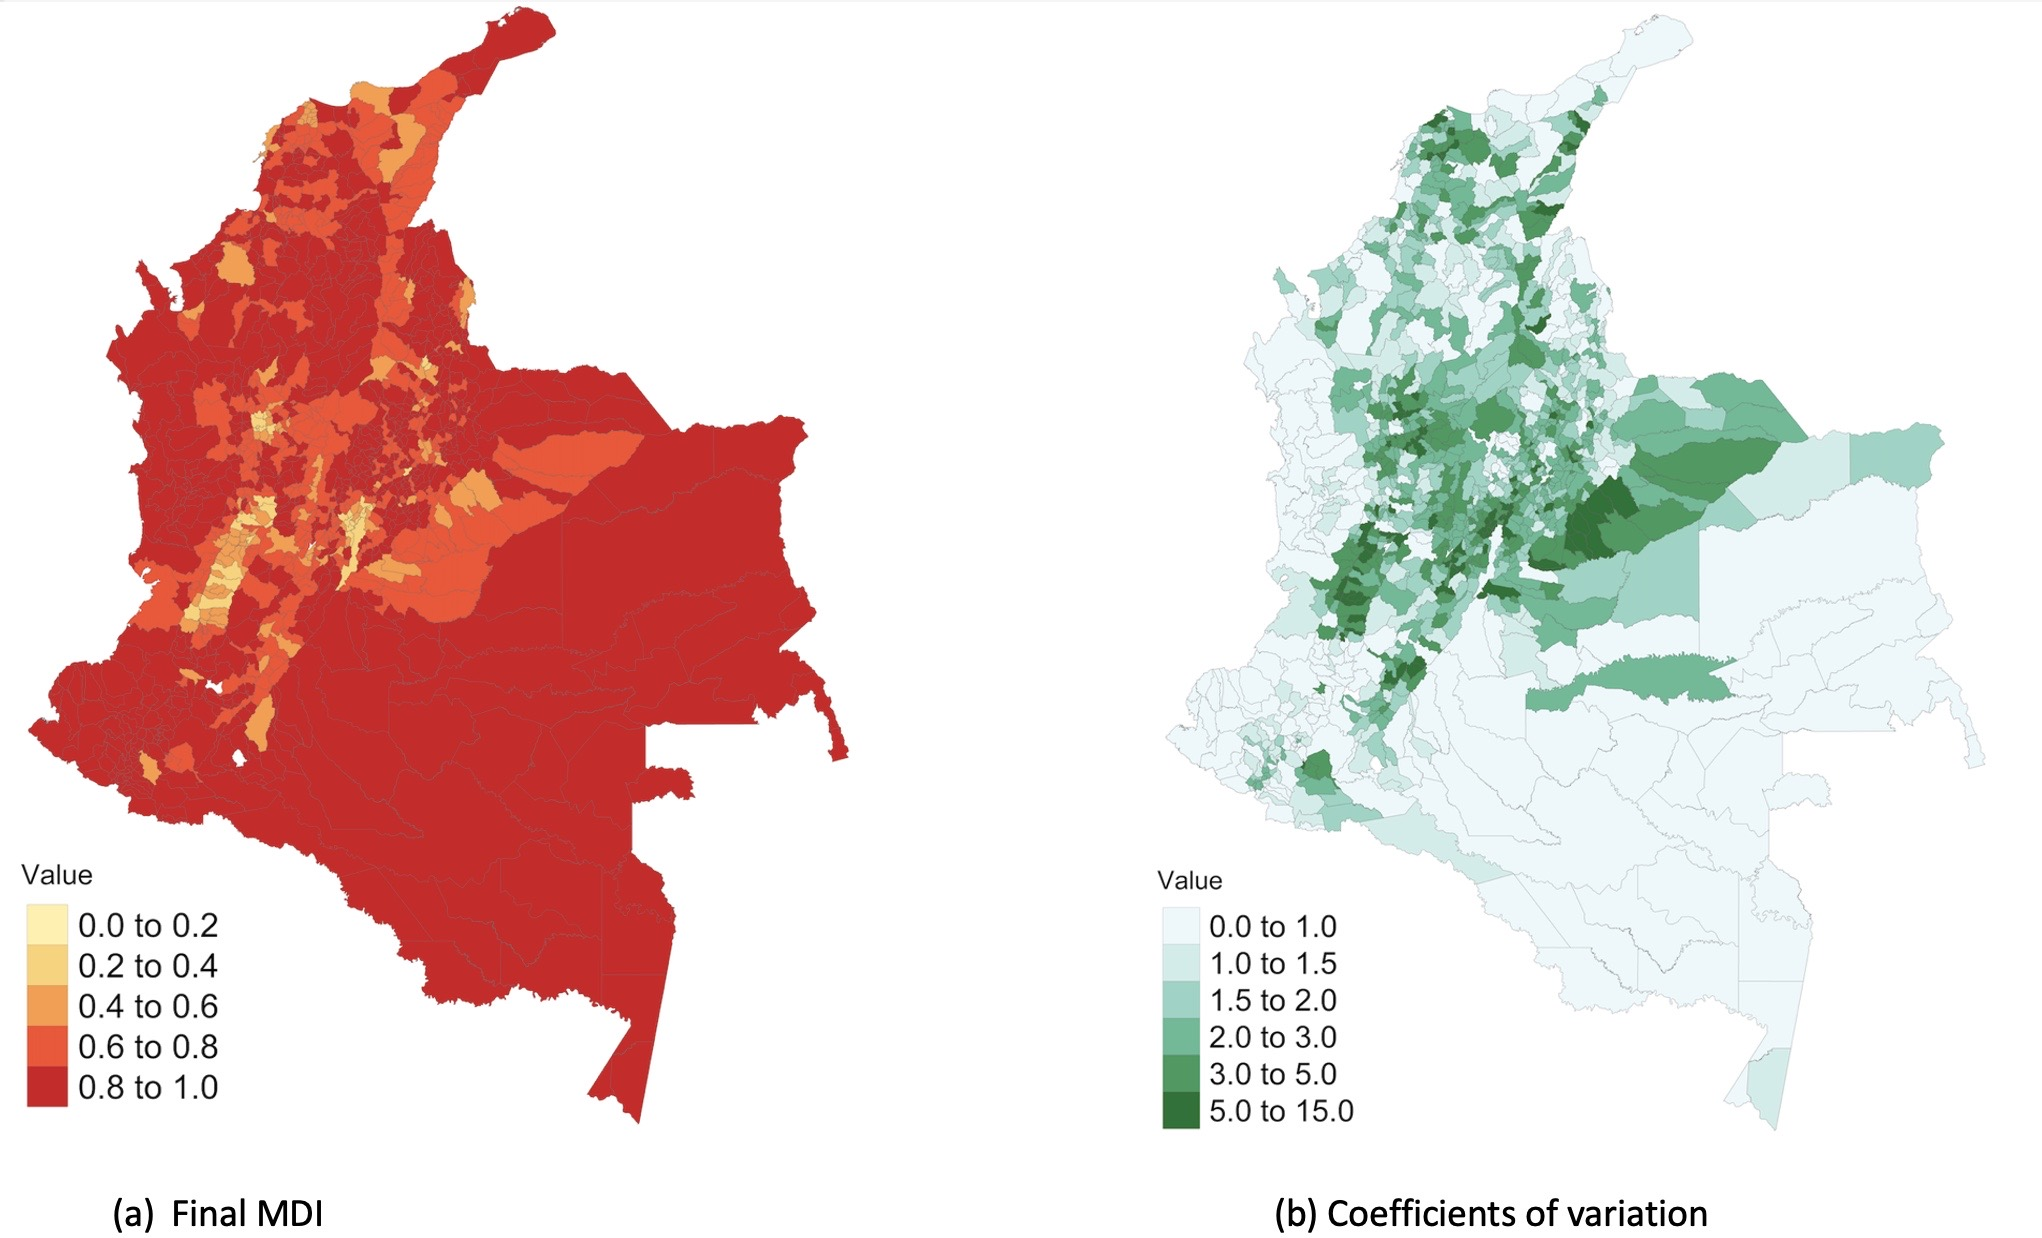
\includegraphics[width=11cm]{Bild 24.09.22 um 17.42.jpg}
    \caption{Model-based estimates for final MDI (a) and coefficients of variation (b) for municipalities in Colombia.}
\end{figure}

\end{frame}

\section{Conclusion}

\frame[noframenumbering]{\tableofcontents[currentsection,hideothersubsections,currentsubsection]}

\begin{frame}{Conclusion and further research}
    
Unit-level Bernoulli logit mixed models can be used when one, two or more indicators of the MDI are not available in the census data. 

    \vspace{0.3cm}

\pause

\textbf{Further research:}

\begin{itemize}
    \item Modeling (co-)relations: How to take into account dependencies and covariances between indicators? and dimensions?
    
        \vspace{0.3cm}
        
    \pause
    
\item Time-gap between census and survey: Modeling all indicators to ``update" them yearly. 

    \vspace{0.3cm}
    
\pause 

\item MSE estimation: Evaluate the performance of the point and variance estimators. 

\vspace{0.3cm}
    
\pause 

\item Benchmark: Possible alternatives and Bayesian approximations.

\vspace{0.3cm}

%\pause 

%\item Find the distribution function of MDI to avoid the Monte Carlo approach in the point estimate.


\pause 

\item Generalization: Compute all the indicators and dimensions of the MDI with SAE methods.

\end{itemize}


\end{frame}

\begin{frame} {Main references}

\begin{itemize}

    \vspace{0.3cm}
    
    \item Chandra H, Kumar S, Aditya K. (2018). Small area estimation of proportions with different levels of auxiliary data. \textit{Biometrical Journal}. 60(2): 395-415.
        \vspace{0.3cm}
        
    \item González-Manteiga, W., Lombardía, M. J., Molina, I., Morales, D., and
Santamaría, L. (2007).
Estimation of the mean squared error of predictors of small area linear parameters
under a logistic mixed model.
\textit{Computational statistics & data analysis}, 51(5): 2720–2733.
        \vspace{0.3cm}
\item Hobza, T., & Morales, D. (2016). Empirical best prediction under unit-level logit mixed models. \textit{Journal of Official Statistics}, 32(3), 661.
        \vspace{0.3cm}
    \item Jiang, J., & Lahiri, P. (2001). Empirical best prediction for small area inference with binary data. \textit{Annals of the Institute of Statistical Mathematics}, 53(2), 217-243.
       \vspace{0.3cm}
    \item Morales, D., Esteban, M. D., Pérez, A., & Hobza, T. (2021). \textit{A course on small area estimation and mixed models. Methods, theory and applications in R.}
\end{itemize}

           
       %\bibliographystyle{apalike}

        %{\footnotesize
%\bibliography{bibfile}}
\end{frame}

\begin{frame}

\vspace{3cm}

\begin{center}
      \textbf{Thank you for your attention}

\vspace{0.5cm}

\textbf{Alejandra Arias-Salazar
    (alejandra.arias@fu-berlin.de)}
    
         \vspace{0.8cm}
     
     \scriptsize{The authors gratefully acknowledge support by UAEU Start-up Research Grant from the United Arab Emirates University}
\end{center}
  


\end{frame}



\appendix
\section{MDI predictor: two missing indicators}\label{AppendixA}
\begin{frame}
\frametitle{MDI predictor: two missing indicators}

\hyperlink{point}{\beamerreturnbutton{Point}}

Finding $W_{j}=\alpha\left(Y_{1j}+Y_{2j}\right)$


The probability mass function of $W_{j}$ is defined by:
\begin{align*}
f\left(W_{j}\right)= & \begin{cases}
\left(1-p_{1}\right)\left(1-p2\right) & \text{if }w_{j}=0,\\
p_{2}\left(1-p_{1}\right)+p_{1}\left(1-p_{2}\right) & \text{if }w_{j}=\alpha,\\
p_{1}p_{2} & \text{if }w_{j}=2\alpha,\\
0 & \text{otherwise}.
\end{cases}
\end{align*}

\begin{enumerate}
\item  Use the sample data to fit a unit-level Binomial logit mixed model for each indicator ($Y_{1j}, Y_{2j}$) and estimate $\hat{\beta}^{Y_1}$, $\hat{\beta}^{Y_2}$, $\hat{u}^{Y_1}_d$ and $\hat{u}^{Y_2}_d$. 

\item For each individual $j$ in the domain $d$ of the census, predict the probability of obtaining the value 1. i.e. $\hat{\pi}^{in,Y_1}_{dj}$ and $ \hat{\pi}^{in,Y_2}_{dj}$. 

\item Define $\delta$, as a fixed threshold that defines the number of deprivations. 

 \item $X_{j}=\alpha\left(Y_{1j}+Y_{2j}\right)+k_{j}$ a general linear combination of the two discrete random variables, with $k_{j}$
a known parameters $\forall j \in U$

\item Using the additive condition proved above, calculate the expectation as the target estimator for each individual
\begin{align*}
\text{MDI}_d=E\left(\bar{Z}_{d}\right).
\end{align*}
\end{enumerate}



\end{frame}

\end{document}